\documentclass{standalone}
\usepackage{tikz}
\begin{document}%
	\begin{tikzpicture}[mylabel/.style={anchor=north west,font=\bfseries, color=black}%
		]
		\node[] at (0, -2) (irbRouter) {\begin{tabular}{c}
				
\includegraphics[width=16pt]{pic/top/router}\\
				IRB-Router\\
		\end{tabular}};
		\node[] at (0, -5) (itmcRouter) {\begin{tabular}{c}
				
\includegraphics[width=16pt]{pic/top/router}\\
				ITMC-Router\\
		\end{tabular}};
		\node[] at (0, -8) (inet) {\begin{tabular}{c}
				
\includegraphics[width=16pt]{pic/top/cloud}\\
				Internet\\
		\end{tabular}};

		\only<1-2>{
		\node[] at (4, -6) (irbSwitch) {\begin{tabular}{c}
			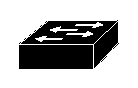
\includegraphics[width=16pt]{pic/top/switch}\\
			\only<1-2>{Switch \\}
		\end{tabular}};
		\node[] at (8, -6) (irbServer) {\begin{tabular}{c}
				
\includegraphics[width=16pt]{pic/top/server}\\
				\only<1-2>{IRB-Server 0$\dots$9\\}
		\end{tabular}};
		
		\node[] at (4, -0) (studentSwitch) {\begin{tabular}{c}
				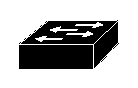
\includegraphics[width=16pt]{pic/top/switch}\\
				\only<1-2>{Switch \\}
		\end{tabular}};
		\node[] at (8, -0) (studentPC) {\begin{tabular}{c}
				
\includegraphics[width=16pt]{pic/top/pc}\\
				\only<1-2>{Studentische PCs 0$\dots$99\\}
		\end{tabular}};
		
		\node[] at (4, -2) (lssSwitch) {\begin{tabular}{c}
				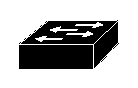
\includegraphics[width=16pt]{pic/top/switch}\\
				\only<1-2>{Switch \\}
		\end{tabular}};
		\node[] at (8, -2) (lss) {\begin{tabular}{c}
				
\includegraphics[width=16pt]{pic/top/pc}\\
				\only<1-2>{Lehrstuhl-1 0$\dots$39\\}
		\end{tabular}};
		
		\node[] at (4, -4) (lseSwitch) {\begin{tabular}{c}
				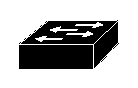
\includegraphics[width=16pt]{pic/top/switch}\\
				\only<1-2>{Switch \\}
		\end{tabular}};
		\node[] at (8, -4) (lse) {\begin{tabular}{c}
				
\includegraphics[width=16pt]{pic/top/pc}\\
				\only<1-2>{Lehrstuhl-14 0$\dots$39\\}
		\end{tabular}};
		
		
		\node[] at (4, -8) (aliceServer) {\begin{tabular}{c}
				
\includegraphics[width=16pt]{pic/top/server}\\
				\only<1-2>{Alice-Server 0$\dots$9\\}
		\end{tabular}};
		}
	
		\node[] at (-4, -8) (eve) {\begin{tabular}{c}
				
\includegraphics[width=16pt]{pic/top/laptop}\\
				Eve\\
		\end{tabular}};
		
		\only<1>{\path[-] (inet) 
			edge (aliceServer)
			edge (eve);
			
			\path[-] (irbRouter) 
			edge  (lssSwitch)
			edge (lseSwitch)
			edge (studentSwitch)
			edge (irbSwitch);
			
			\path[-] (lssSwitch) edge  (lss);
			\path[-] (lseSwitch) edge  (lse);
			\path[-] (studentSwitch) edge (studentPC); 
			\path[-] (irbSwitch) edge  (irbServer);
			
			\draw[dotted] (lssSwitch) 
			edge (lseSwitch)
			edge (lse);
			\draw[dotted] (lss) 
			edge (lseSwitch)
			edge (lse);
		}
		
		\path[-] (irbRouter) 
		edge (itmcRouter);
		\path[-] (itmcRouter)
		edge (inet);
		
		\only<2->{
			\draw[draw=gray, dotted, red, thick] (2,1) rectangle node[pos=.1, anchor=north west, align= right, black] {
				\only<3->{
					\textbf{Client Bereich} \\ \\	
					{
						{\begin{varwidth}{\linewidth}\begin{itemize}
									\item TCPBasicClientApp\hfill\tikzmark{a}
									\item UDPVideoStreamCli
									\item UDPBasicApp
									\item PingApps\hfill\tikzmark{b}
						\end{itemize}\end{varwidth}}
						\mybrace{a}{b}[4-5-Anwendungen]
					}
				}
			} (12, -4.9);
			\draw[draw=gray, dotted, blue, thick] (2,-5.1) rectangle node[pos=.1, anchor=north west, align= right, black] {
				\only<3->{
					\textbf{Server Bereich} \\ \\
					{
						{\begin{varwidth}{\linewidth}\begin{itemize}
									\item Alle Client Apps\hfill\tikzmark{c}
									\item TCPGenericSrvApp
									\item UDPVideoStreamSvr
									\item UDPEchoApp\hfill\tikzmark{d}
						\end{itemize}\end{varwidth}}
						\mybrace{c}{d}[50-100 Anwendungen]
					}
				}
			} (12, -9);
		
		
			\only<3->{
				\path[-] (inet) 
				edge (eve);
				
				\path[-, dashed] (irbRouter) 
				edge (2, -2)
				edge (2, -5.1);
				
				\path[-, dashed] (inet) 
				edge (2, -8);
			}
		
%			\only<4->{
%				\draw[draw=white, dotted] (-9,1) rectangle node[pos=.1, anchor=north west, align= center] {
%						\textbf{Allgemein} \\ \\
%						{
%							{\begin{varwidth}{\linewidth}\begin{itemize}
%								\item Linux-TCP-Konfiguration
%								\item 3 ARP-Versuche
%								\item Internet 
%								\begin{itemize}
%									\item RTT $\sim$ 70 ms
%									\item Drop $\sim$ 0.001 \% 
%								\end{itemize}
%							\end{itemize}\end{varwidth}}
%						}
%				} (-2, -6);
%			}
		}
	
		\only<1>{
			\path[-] (inet) 
			edge node[midway, above] {\footnotesize $\infty$ \si{\giga\bit\per\second}} (aliceServer)
			edge node[midway, above] {\footnotesize $\infty$ \si{\giga\bit\per\second}} (eve);
			
			\path[-] (irbRouter) 
			edge node[midway, left] {\footnotesize 40 \si{\giga\bit\per\second}} (itmcRouter);
			\path[-] (itmcRouter)
			edge node[midway, left] {\footnotesize 10 \si{\giga\bit\per\second}} (inet);
			
			\path[-] (irbRouter) 
			edge node[midway, above, sloped] {\footnotesize 10 \si{\giga\bit\per\second}} (lssSwitch)
			edge node[midway, above, sloped] {\footnotesize 10 \si{\giga\bit\per\second}} (lseSwitch)
			edge node[midway, above, sloped] {\footnotesize 10 \si{\giga\bit\per\second}} (studentSwitch)
			edge node[midway, above, sloped] {\footnotesize 40 \si{\giga\bit\per\second}} (irbSwitch);
			
			\path[-] (lssSwitch) edge node[midway, above] {\footnotesize 1 \si{\giga\bit\per\second}} (lss);
			\path[-] (lseSwitch) edge node[midway, above] {\footnotesize 1 \si{\giga\bit\per\second}} (lse);
			\path[-] (studentSwitch) edge node[midway, above] {\footnotesize 1 \si{\giga\bit\per\second}} (studentPC); 
			\path[-] (irbSwitch) edge node[midway, above] {\footnotesize 10 \si{\giga\bit\per\second}} (irbServer);
			
			\draw[dotted] (lssSwitch) 
			edge (lseSwitch)
			edge (lse);
			\draw[dotted] (lss) 
			edge (lseSwitch)
			edge (lse);
		}
	
		\only<2>{
			\path[-] (inet) 
			edge  (aliceServer)
			edge  (eve);
			
			\path[-] (irbRouter) 
			edge  (itmcRouter);
			\path[-] (itmcRouter)
			edge  (inet);
			
			\path[-] (irbRouter) 
			edge (lssSwitch)
			edge (lseSwitch)
			edge (studentSwitch)
			edge (irbSwitch);
			
			\path[-] (lssSwitch) edge (lss);
			\path[-] (lseSwitch) edge (lse);
			\path[-] (studentSwitch) edge (studentPC); 
			\path[-] (irbSwitch) edge (irbServer);
			
			\draw[dotted] (lssSwitch) 
			edge (lseSwitch)
			edge (lse);
			\draw[dotted] (lss) 
			edge (lseSwitch)
			edge (lse);
		}
	
		%Hidden Nodes
		\node[] at (-4, 2) {}; 
		\node[] at (12,-9) {}; 
	\end{tikzpicture}%
\end{document}